\documentclass{tufte-handout}

\title{CS294: Deep Reinforcement Learning
       \thanks{Course Instructors: Sergey Levine} \\
       \Large Lecture Notes: Introduction to Policy Gradient \thanks{Author: InnerPeace}}

\date{Fall 2017\thanks{Un-official Lecture Notes}} % without \date command, current date is supplied


%\geometry{showframe} % display margins for debugging page layout

\usepackage{graphicx} % allow embedded images
  \setkeys{Gin}{width=\linewidth,totalheight=\textheight,keepaspectratio}
  \graphicspath{{notes2/fig/}} % set of paths to search for images
\usepackage{amsmath}  % extended mathematics
\usepackage{amstext}  % extended text
\usepackage{booktabs} % book-quality tables
\usepackage{units}    % non-stacked fractions and better unit spacing
\usepackage{multicol} % multiple column layout facilities
\usepackage{lipsum}   % filler text
\usepackage{xcolor}
\usepackage{fancyvrb} % extended verbatim environments
\usepackage{placeins}
  \fvset{fontsize=\normalsize}% default font size for fancy-verbatim environments

% Standardize command font styles and environments
\newcommand{\doccmd}[1]{\texttt{\textbackslash#1}}% command name -- adds backslash automatically
\newcommand{\docopt}[1]{\ensuremath{\langle}\textrm{\textit{#1}}\ensuremath{\rangle}}% optional command argument
\newcommand{\docarg}[1]{\textrm{\textit{#1}}}% (required) command argument
\newcommand{\docenv}[1]{\textsf{#1}}% environment name
\newcommand{\docpkg}[1]{\texttt{#1}}% package name
\newcommand{\doccls}[1]{\texttt{#1}}% document class name
\newcommand{\docclsopt}[1]{\texttt{#1}}% document class option name
\newenvironment{docspec}{\begin{quote}\noindent}{\end{quote}}% command specification environment
\newcommand{\argmin}{\operatornamewithlimits{argmin}}
\newcommand{\argmax}{\operatornamewithlimits{argmax}}
\newcommand{\textunderscript}[1]{$_{\text{#1}}$}

\newcommand{\etal}{\textit{et al}. }
\newcommand{\ie}{\textit{i}.\textit{e}., }
\newcommand{\eg}{\textit{e}.\textit{g}. }
\newcommand{\s}{\mathbf{s}}
\newcommand{\act}{\mathbf{a}}

\setcounter{secnumdepth}{3}

\begin{document}

\maketitle% this prints the handout title, author, and date

%\printclassoptions


\textbf{Keyphrases: Markov Decision Process. Reinforcement Learning Algorithms.}

This set of notes first introduces the definition of Markov Decision Process (MDP). Then it dives into the definition of RL problems and goals, also giving the high-level overview of the anatomy of RL which is the high-level structure shared among all the algorithms we will learn. Lastly we give a brief overview of RL algorithm types.

\section{Reward Function}

In \emph{Imitation Learning}, we learned how to train the policy with demonstrations. But how can we achieve the result without using example data? Following the mechanism of solving typical DL problem, we need to find a way to define the task, and find out what the object function is, then we may apply SGD trick to learn the policy. In RL, we usually take the rewards $r(\mathbf{s}, \mathbf{a})$ \thanks{Some may also use the notation $c(\mathbf{x}, \mathbf{u}) $ as the cost function, where $r(\mathbf{s}, \mathbf{a}) = -c(\mathbf{x}, \mathbf{u}) $ } of all time-steps as the object function, which tells us which states and actions are preferred. In the case of driving, one has high reward when driving safely on the road with desire speed or low reward for being a state where one collided with another car. The crucial thing is that the reward function does not tell you how to act right now, it represents the desirability of the outcome. The the job of RL is trying to take a preferred action so that the future outcome will be more desirable which is referred as \emph{delayed reward problem}.

\begin{marginfigure}
  \centering
  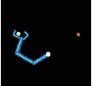
\includegraphics[width=\linewidth]{robotic_arm}
  \caption{simple benchmark simulation task}
  \label{fig:robotic_arm}
\end{marginfigure}

What the reward function should be? As the case of a simple benchmark simulation task where the robotic arm trying to grab a little ball and move to a specific spot (figure \ref{fig:robotic_arm}), the reward function is straightforward in theory.

$$
r(\mathbf{s}, \mathbf{a}) = \begin{cases}
1 \quad \text{if object at target} \\
0 \quad \text{otherwise}
\end{cases}
$$

However, with the kinds of RL algorithms we have for now, reward function like this is very difficult to work with. The reason is that until you move the ball to the target, you don't know what you are supposed to be doing. So in practice, we usually end up with a much more complex reward function doing the seemingly simple thing, \eg minimizing the distance between the gripper and object, the distance between object and target, also the size of actions in case of taking gigantic torques on the joints.

\begin{align*}
r(\mathbf{s}, \mathbf{a}) =
& - w_1 || p_{gripper} (\mathbf{s}) - p_{object}(\mathbf{s}) || ^ 2  + \\
& - w_2 || p_{object} (\mathbf{s}) - p_{target}(\mathbf{s}) || ^ 2  + \\
& - w_3 || \mathbf{a} || ^2
\end{align*}

The reward function reconstructing for practical use sometimes is referred as \emph{reward shaping} \thanks{Refer Ng's \href{http://rll.berkeley.edu/deeprlcourse/docs/ng-thesis.pdf}{\underline{thesis}} for more details}. For imitation learning, the reward function is the log probability of action given state. The problem is that we often do not know what the reward is in real life scenario, \eg pouring water into a cup, and we will learn some methods to mitigate this problem, \ie learning the reward with Inverse Reinforcement Learning.

\[
r(\mathbf{s}, \mathbf{a}) = \log p(\mathbf{a} = \pi ^\star (\mathbf{s}) | \mathbf{s})
\]

A note about terminology of "R" word. In computer science, RL is often referred as the \emph{problem} statement where the goal is $\max \sum_{t=1}^T E[r(\mathbf{s}_t, \mathbf{a}_t)] $ where $\mathbf{s}_{t+1} \sim p(\mathbf{s}_{t+1} | \mathbf{s}_{t}, \mathbf{a}_{t}) $. However, in optimal control or dynamic programming, RL represents the \emph{method} which does not use the \emph{model} $\max \sum_{t=1}^T E[r(\mathbf{s}_t, \mathbf{a}_t)] $.


\section{Markov Decision Process}

The state, action, reward and transition probability together define the \emph{Markov Decision Process (MDP)}.

\subsection{Markov Chain}

Markov Chain is the formalism for reasoning about a particular kind of stochastic process. It's defined by state space $\mathcal{S}$ and transition operator $\mathcal{T}$ as $\mathcal{M} = \{\mathcal{S}, \mathcal{T} \}$. For states ${s} \in \mathcal{S}$, it could be discrete or continuous, \ie
a categorical variable or a vector of continuous numbers. $\mathcal{T}$ defines the probability of transferring to a new state give current state, $p({s}_{t+1} | {s}_{t})$. Let's assume that the state is discrete, and let $\mu_{t,i} = p(s_t = i) $, \ie the probability of being state i at timestep t, so
$\vec{\mu}_t $ is a vector of probabilities. Let $\mathcal{T}_{i,j} = p(s_{t+1} = i | s_t = j) $, then ${\vec{\mu}}_{t+1} = \mathcal{T} \vec{\mu}_{t}$ where
$\mathcal{T}$ is just a linear operator. If the state is continuous, then the $\mathcal{T}$ becomes infinitely large linear operator. The transition process demonstrates the independent property where $\vec{\mu_{t+1}} $ only depend on $\vec{\mu_t} $. And the second order or third order Markov chain means that it depends on the current and previous one, or the one before that.

\begin{marginfigure}
  \centering
  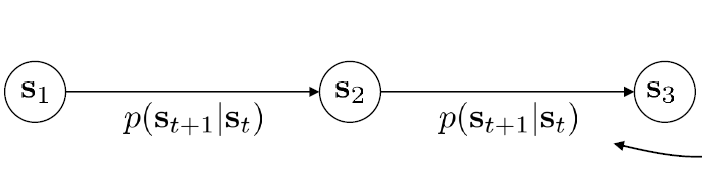
\includegraphics[width=\linewidth]{mchain}
  \caption{Markov Chain}
  \label{fig:mchain}
\end{marginfigure}

\subsection{Markov Decision Process}

MDP is an extension of Markov Chains to decision making setting. MDP is defined as $\mathcal{M}=\{\mathcal{S}, \mathcal{A}, \mathcal{T}, r \} $, the state space is same as Markov Chain, and the action space $\mathcal{A}$ is alike where $ a \in \mathcal{A}$ could be discrete or continuous. The transition operator $\mathcal{T}$ becomes a tensor (3 dimension) which describes the probability of entering a particular state given current state and action.
\begin{align*}
 \mu_{t,j} &= p(s_t = j) \\
 \xi_{t, k} &= p(a_t = k) \\
 \mathcal{T}_{i,j,k} &= p(s_{t+1} = i | s_t = j, a_t = k) \\
 \mu_{t+1,i} &= \sum_{j,k} \mathcal{T}_{i,j,k} \mu_{t,j} \xi_{t,k}
\end{align*}

And lastly, the reward function $r: \mathcal{S} \times \mathcal{A} \to \mathbb{R}$ which maps state and action to real value numbers, and $r(s_t, a_t) $ is the reward of state and action pair at a particular timestep t.

Another generalization of Markov Chain is \emph{Partially Observed Markov Decision Process (POMDP)} which is defined as
$\mathcal{M} = \{\mathcal{S}, \mathcal{A}, \mathcal{O}, \mathcal{T}, \mathcal{E}, r \} $. We alluded observation in Imitation learning, and $\mathcal{O}$
represents the observation space, observations $o \in \mathcal{O}$ could also be discrete or continuous. $\mathcal{E}$ means the emission probability
 $p(o_t, s_t)$ tells how likely a certain observation $o$ to occur given state $s$ at timestep $t$.

\marginnote{\textbf{Markov Decision Process:} \\
(Adapted from cs231n of stanford.)
At time step $t=0$, environment samples initial state $s_0 \sim p(s_0)$.
\begin{itemize}
\item [Then for $t=0$ until done:]
\item Agent selects action $a_t$
\item Environment gets reward $r(s_t, a_t) $
\item Environment samples next state $s_{t+1} \sim p(s_{t+1} | s_t, a_t) $
\item Agent receives reward $r_t$ and next state $s_{t+1}$
\end{itemize}
}

\section{The Goal}

In RL problem setting, we have a initial state $\s_1$ and the parametrized policy $\pi_\theta(\act|\s)$ \thanks{For now we focus on the fully observed case.} output the action $\act_1$, then with transition function $p(\s' | \s, \act)$ which we usually do not know, we enter a new state $\s'$ and keep circling following the mechanism.

\begin{figure*}
  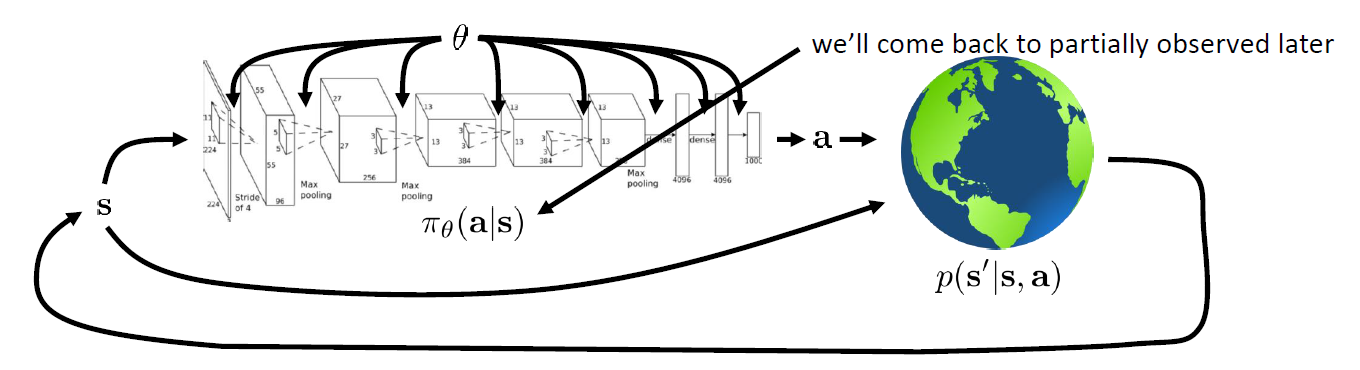
\includegraphics[width= 10cm]{goal}
  \caption{Illustration of RL problem setting}
  \label{fig: goal}
\end{figure*}

This process gives rise to the distribution over state-action sequences for finite horizon task. The distribution is given by the probability of the starting point $\s_1$ which is often determined by nature, times the product of all the timesteps of probability of taking an action times the probability of transitioning to the next state. We will denote the joint probability over $T$ states and actions as $p_\theta(\tau)$ where $\tau$ is the trajectory of states and actions, and the probability depends on $\theta$.
\[
\underbrace{p_\theta(\s_1, \act_1, \cdots , \s_T, \act_T)}_{\pi_\theta (\tau)} =
  p(\s_1) \prod _{t=1}^T \big(\pi_\theta (\act_t | \s_t) p(\s_{t+1} | \s_t, \act_t)\big)
\]

Then the objective of RL problem setting could be finding the parameter $\theta$ which maximize the expectation of the overall rewards w.r.t trajectories drawn from probability distribution $p_\theta(\tau)$. And the policy gives rise to trajectory distributions.

\[
\theta^\star = \arg \max_\theta E_{\tau \sim p_\theta(\tau) }\Big[ \sum_t r(\s_t, \act_t) \Big]
\]

The transition probability and policy at timestep $t$ could be seen as \emph{Markov Chain} on $(\s, \act)$, where
\[
p((\s_{t+1}, \act_{t+1}) | (\s_{t}, \act_t)) =
  p(\s_{t+1} | \s_t, \act_t) \pi_\theta(\act _{a+1} | \s_{t+1})
\]

or
\[
  \begin{pmatrix}
  \s_{t+1} \\ \act_{t+1}
  \end{pmatrix} = \mathcal{T}
  \begin{pmatrix}
  \s_{t} \\ \act_{t}
  \end{pmatrix}
\]

The probability \emph{state-action} of the next timestep is given by $\mathcal{T}$ times the probability of that at current timestep. $\mathcal{T}$ is the \emph{state-action} transition operator.
We can turn MDP into the Augmented Markov Chain with knowing the policy, which is helpful to define the infinite horizon task. With turning into Markov Chain, we can rewrite the objective as.
\begin{align*}
\theta^\star & = \arg \max_\theta E_{\tau \sim p_\theta(\tau) }\Big[ \sum_t r(\s_t, \act_t) \Big] \\
            & = \arg \max_\theta \sum_{t=1} ^ T E_{(\s_t, \act_t)\sim p_\theta (\s_t, \act_t)} \big[r(\s_t, \act_t) \big]
\end{align*}


We take the sum outside of the expectation cause the expectation is linear, and change to calculate the expectation over reward of timestep t, and sum over them all afterwards. The $(\s_t, \act_t)$ is drawn from the state-action marginal distribution $p_\theta (\s_t, \act_t)$.

Since the \emph{state-action} transition operator is linear, we could obtain the probability for timestep $t+k$.
\[
  \begin{pmatrix}
  \s_{t+k} \\ \act_{t+k}
  \end{pmatrix} = \mathcal{T}^k
  \begin{pmatrix}
  \s_{t} \\ \act_{t}
  \end{pmatrix}
\]

When timesteps $T$ goes to infinite, does  $p(\s_t, \act_t)$ converge to a \emph{stationary} distribution? Firstly, let's assume the stationary distribution $\mu$ exists, which stays the same before and after the transition.
\[
  \mu = \mathcal{T} \mu \quad \to \quad (\mathcal{T} - \mathbf{I}) \mu = 0
\]

It's true when $\mu$ is eigenvector of $\mathcal{T}$ with eigenvalue 1. And if $\mathcal{T}$ is a stochastic matrix under some regularity conditions, then
$\mu$ does exist.  Which means the marginal distribution will finally converge the stationary distribution $\mu = p_\theta (\s, \act)$. Then for the infinite case, we divide the sum with overall time-steps $T$ since the sum over rewards of infinite time-steps also goes to infinite. At the same time, the distribution over state-action will be dominated by stationary distribution when $T$ becomes infinite, \eg after 5 million steps, it converge to stationary distribution, and since you have infinite long life time, the first 5 million steps won't matter anymore.
\begin{align*}
\theta^\star &= \arg \max_\theta \frac{1}{T} \sum_{t=1} ^ T E_{(\s_t, \act_t)\sim p_\theta (\s_t, \act_t)} \big[r(\s_t, \act_t) \big] \\
& =\arg \max_\theta E_{(\s, \act)\sim p_\theta (\s, \act)} \big[r(\s, \act) \big]
\end{align*}

The objective reduce to just the expectation under stationary distribution.

In RL, we almost always care about \emph{expectations}. In some cases, the reward is discrete, \eg the task showed in figure \ref{fig:robotic_arm}
where the reward could be 1 when completing the task or 0 otherwise. With \emph{expectation} over large amounts of trials, we can introduce the probability
of success or failure which will smooth the objective so that we can applied gradient based methods to learn the policy.

\section{Anatomy}

In general, all the algorithms consist of three parts: {\color{orange} samples generating}, {\color{green} model fitting or return estimating},
{\color{blue} policy improving}.

Samples generating is the process of sampling the trajectories with running the current policy. And it could be expensive for the real time experiments, or trivial in simulator which could be thousands times faster.

Model fitting or return estimating is computing delayed rewards from current time-step $\hat{Q}=\sum_{t'=t}^T \gamma ^{t'-t} r_{t'} $, which is trivial and fast, for policy gradient algorithm, fitting $Q_\phi(\s, \act) $ which is expensive but non-trivial to parallelize for actor-critic and Q-learning algorithm and estimating $p(\s' | \s, \act) $ for model-based algorithms.

Policy improving could be gradient updating for PG, computing $\pi(\s) = \arg \max Q_\phi (\s, \act)$ which is trivial for Q-learning or optimizing $\pi_\theta(\act | \s) $ in model-based algorithms which is more expensive.

\begin{marginfigure}
  \centering
  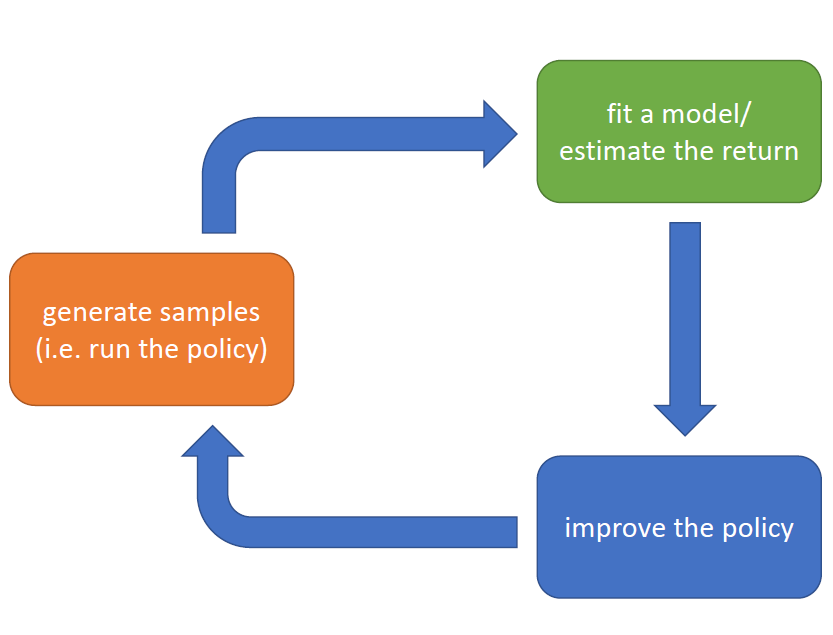
\includegraphics[width=\linewidth]{anatomy}
  \caption{The anatomy of RL algorithms}
  \label{fig:anatomy}
\end{marginfigure}

In order to work with stochastic systems, we use the conditional expectations where the objective is to maximize the overall rewards for the policy. We can decouple the state-action distribution to state distribution and action distribution respectively.

\begin{align*}
R & = \sum_{t=1} ^ T E_{(\s_t, \act_t)\sim p_\theta (\s_t, \act_t)} \big[r(\s_t, \act_t) \big] \\
  & = E_{\s_1 \sim p(\s_1)} \Big[E_{\act_1 \sim \pi(\act_1 | \s_1)} [Q(\s_1, \act_1) | \s_1] \Big] \\
Q(\s_1, \act_1) & = r(\s_1, \act_1) + E_{\s_2 \sim p(\s_2)} \Big[E_{\act_2 \sim \pi(\act_2 | \s_2)} [r(\s_2, \act_2) + \cdots | \s_2] | \s_1, \act_1 \Big]
\end{align*}

Then it's easy to modify $\pi_\theta(\act_1 | \s_1) $ if $Q(\s_1, \act_1)$ is known, \eg set $\pi_{\theta'}(\act | \s) = 1$ if
$ \act = \arg \max_{\act} Q^{\pi_\theta}(\s, \act)$, the improved policy is at least as good as $\pi_\theta$.

\subsection{Q-function}

We define the \emph{Q-function} $Q^\pi(\s_t, \act_t)$ as the conditional expected cumulative reward from taking action $\act_t$ in state $\s_t$ and then following the policy, which specifies how good a state-action pair is.
\[
Q^\pi (\s_t, \act_t) = \sum_{t'=t}^T E_{\pi_\theta} [r(\s_{t'}, \act_{t'}) | \s_t, \act_t]
\]

\subsection{Value function}
Similarly, we specify how good a state is with \emph{value function}, which is defined as the expected cumulative reward from state $\s_t$ conditioned on the policy $\pi$.
\[
V^\pi (\s_t) = \sum_{t'=t}^T E_{\pi_\theta} [r(\s_{t'}, \act_{t'}) | \s_t]
\]

Then relationship between Q-function and value function is
\[
V^\pi (\s_t) = E_{\act_t \sim \pi(\act_t | \s_t)} Q^\pi (\s_t, \act_t)
\]

And the RL objective could be rewrite as
\[
E _{\s_1 \sim p(\s_1) }[V^\pi (\s_1)]
\]

These functions basically compress all the future rewards from the current state or action, and it helps a lot to improve the policy.

\subsection{Bellman equation}
We define the optimal Q-function $Q^\star$ as the maximum expected cumulative reward achievable from a given state-action pair $(\s, \act)$.
\[
Q^{\pi^\star} (\s_t, \act_t) =\max_\pi \sum_{t'=t}^T E_{\pi_\theta} [r(\s_{t'}, \act_{t'}) | \s_t = \s, \act_t = \act]
\]

$Q^{\pi^\star}$ satisfies the \emph{Bellman equation}:
\[
Q^{\pi^\star} (\s, \act) =E_{\s' \sim p(\s' | \s, \act)} \Big[r + \max_{\act'}  Q^{\pi^\star}(\s', \act') | \s, \act \Big]
\]

The intuition is that if the optimal state-action values for the next time-step $Q^{\pi^\star}(\s', \act')$ are known, then the optimal strategy is to take
the action that maximizes the expected value of $r + Q^{\pi^\star}(\s', \act')$. And the optimal policy $\pi^\star$ corresponds to taking the best action in any state as specified by $Q^{\pi^\star}$. This is the principle of Q-learning, and we will learn more about it.

Another way to take advantage of Q-functions and value functions is computing gradient to increase probability of good action $\act$. Since
$V^\pi (\s_t) = E[Q^\pi(\s_t, \act_t)]  $, if $Q^\pi(\s_t, \act_t) > V^\pi (\s_t)$, then $\act$ is better than average. Then we can modify policy $\pi$
to increase probability of $\act$.

\section{Algorithms}

\subsection{Policy Gradient}

Policy Gradient directly differentiate the objective of RL problem, and improve the policy with tricks like SGD, and optimizer like \emph{adam}
also works fine. Firstly, we evaluate returns $R_\tau = \sum_t r(\s_t, \act_t) $ and update parameters of policy network with gradients of returns with respect to parameters $\theta$.
\begin{itemize}
  \item[\textbf{Examples}]
  \item REINFORCE
  \item Natural Policy Gradient
  \item Trust Region Policy Optimization
\end{itemize}

\subsection{Value-based algorithms}
This kind of algorithm has no explicit policy, instead estimating the value function or Q-function of the optimal policy. After sample generating, it tries to fit $V(\s)$ or $Q(\s, \act) $ and set $\pi(\s) =\arg \max_a Q(\s, \act) $ to improve the policy.
\begin{itemize}
  \item[\textbf{Examples}]
  \item Q-learning, DQN
  \item Temporal difference learning
  \item Fitted value iteration
\end{itemize}

\subsection{Actor-critic algorithms}
Actor-critic could be seen as the combination of PG and value-based algorithms which estimate value function or Q-function of the current policy, and use it to import policy with gradient updating. Specifically, it will fit $V(\s) $ or $Q(\s, \act)$, then evaluate the returns with $V$ or $Q$ instead of the cumulative rewards, and finally update policy parameters with gradients. The typical example is \emph{Asynchronous advantage actor critic (A3C)}.

\subsection{Model-based algorithms}
The model-based RL is about estimating the transition model which is used for planning with no explicit policy or to improve the policy with gradients. The model fitting phrase is learning $p(\s_{t+1} | \s_t, \act_t) $, then a few options for the phrase of policy improving.
\begin{itemize}
  \item [\textbf{Use the model to plan}]
  \item Trajectory optimization or optimal control which is primarily used in continuous spaces, both of them are essentially backpropagation to optimize over actions (no explicit policy).
  \item Discrete planning in discrete action spaces, \eg Monte Carlo Tree Search.

  \item [\textbf{Backpropagation gradients into the policy}]
  \item [\textbf{Use the model to learn value function}]
  \item Dynamic programming
  \item Generate simulated experience for model-free learner, \eg \emph{Dyna}.
\end{itemize}

The typical examples is \emph{Dyna} and \emph{Guided Policy Search}.

\subsection{Trade-offs}
In general deep learning setting, \eg supervised learning, where we usually use some flavor of gradient descent and while we may argue about whether SGD with momentum or Adam is better, they are all essentially similar to each other. However, in RL, different algorithms have different trade-offs and there is no algorithm performs best in all cases. So what are the trade-offs?

\textbf{Sample efficiency}: it refers to how many samples we need to generate to learn a good policy. We usually divide RL algorithms into two parts: \emph{on} policy or \emph{off} policy w.r.t the sampling procedure.
\begin{itemize}
  \item Off-policy means that the algorithms are able to improve the policy without generating new samples from that policy.
  \item On-policy means we need to generate new samples \emph{each time} the policy is changed, even a little bit. It's could be problematic for gradient based methods, cause each update changes the policy little bit and you end up with generating so many samples during training.
\end{itemize}

\begin{figure*}
  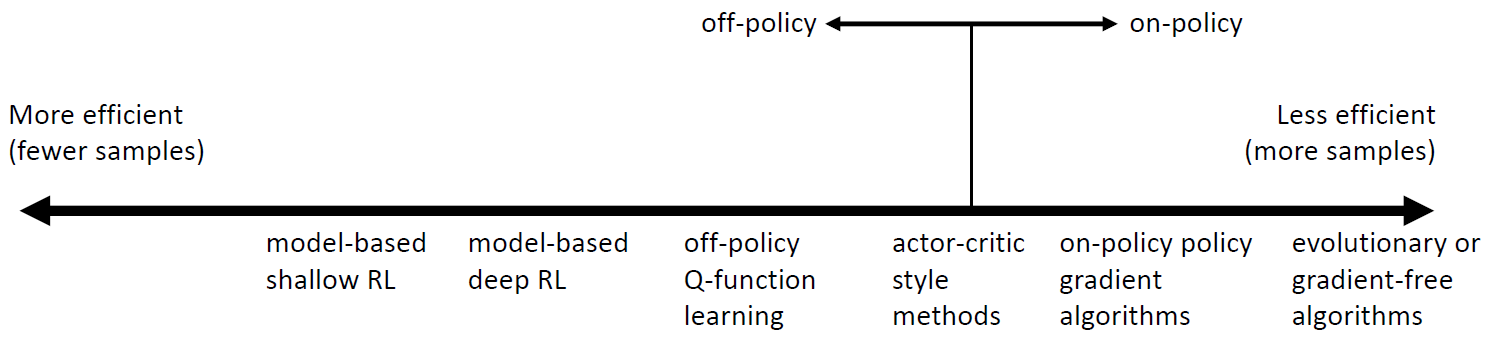
\includegraphics[width=15cm]{sample_efficiency}
  \caption{General Comparison of sample efficiency}
  \label{fig:sample-efficiency}
\end{figure*}

The evolutionary or gradient-free algorithms take no use of the gradients of policy, treat the parameters as black-box or potentially non-differentiable and operates directly on the parameters. To be clear, less efficiency is not synonymous with bad and we may need this kinds of algorithms in some cases, \eg you have fast simulators and with parallelism so that they could be the fastest in terms of the \emph{wall clock time}. In contrast, on-policy policy gradient method is more efficient due to using the gradients. The actor-critic style methods could be off-policy or on-policy which are more efficient. The model-based algorithms perform better w.r.t sample efficiency, specifically, shallow RL is the most efficient by using different approximator like Bayesian function, but typically at the cost of introducing additional assumptions or restricted solvable classes of problems. To be clear that \emph{wall clock time} is not the same as efficiency due to the tricks like working with simulators or parallelism, besides \emph{wall clock time} contains the model fitting or neural network fitting process. Surprisingly, the comparison of efficiency w.r.t the wall clock time looks like the opposite of this figure
\ref{fig:sample-efficiency}.

\textbf{Stability \& ease of use}: it refers to how difficult the algorithm is to choose the hyper-parameters, the learning rates or exploration parameters etc. to get it working. Convergence is the crucial question for learning algorithms, it's always gradient descent for supervised learning, for which convergence is heavily studied and almost guaranteed, but it's often not gradient descent for RL algorithms.
\begin{itemize}
  \item Q-learning is an instance of fixed point iteration. Under certain conditions, it can converge to the optimal expected reward. Approximating expected rewards accurately is not the same as having a good policy. In other words, it's minimizing the error of prediction, not maximizing the expected reward. Sadly, many popular deep RL value fitting algorithms are not guaranteed to converge to anything in the nonlinear case.
  \item For model-based RL, the model is optimized for fitting the physics of the real world, which has complex implications on the performance of the corresponding police, instead of expected reward. Usually the model is trained to predict the future which will converge, but converge to a prediction model which is not equal to better policy.
  \item Policy gradient performs gradient descent or ascent on the true objective, but has other trade-offs.

\end{itemize}

Also, different algorithms hold different assumptions. some will assume stochastic dynamics and stochastic policies, while some would operate better on deterministic dynamics, and the same goes to continuous setting versus discrete cases, episodic setting versus infinite horizon. \eg full observability assumption is generally assumed by value function fitting methods, for the partially observed case, it can mitigated by adding recurrence.  Besides, the performance could be task specific, \eg it's easier to represent the policy, value functions or transition model.

% \begin{table}[ht]
%   \centering
%   \fontfamily{ppl}\selectfont
%   \begin{tabular}{lll | lll}
%     \toprule
%     Model & Dimension & Size & Semantics & Syntax & Total \\
%     \midrule
% 	ivLBL & 100 & 1.5B & 55.9 & 50.1 & 53.2 \\
% 	HPCA & 100 & 1.6B & 4.2 & 16.4 & 10.8\\
% 	GloVE & 100 & 1.6B & 67.5 & 54.3 & 60.3\\
% 	\hline
% 	SG & 300 & 1B & 61 & 61 & 61\\
% 	CBOW & 300 & 1.6B & 16.1 & 52.6 & 36.1\\
% 	vLBL & 300 & 1.5B & 54.2 & 64.8 & 60.0\\
% 	ivLBL & 300 & 1.5B & 65.2 & 63.0 & 64.0\\
% 	GloVe & 300 & 1.6B & 80.8 & 61.5 & 70.3\\
% 	\hline
% 	SVD & 300 & 6B & 6.3 & 8.1 & 7.3\\
% 	SVD-S & 300 & 6B & 36.7 & 46.6 & 42.1\\
% 	SVD-L & 300 & 6B & 56.6 & 63.0 & 60.1\\
% 	CBOW & 300 &6B & 63.6 & 67.4 & 65.7\\
% 	SG & 300 & 6B & 73.0 & 66.0 & 69.1\\
% 	GloVe & 300 & 6B & 77.4 & 67.0 & 71.7\\
% 	\hline
% 	CBOW & 1000 & 6B & 57.3 & 68.9 & 63.7\\
% 	SG & 1000 & 6B & 66.1 & 65.1 & 65.6\\
% 	SVD-L & 300 & 42B & 38.4 & 58.2 & 49.2\\
% 	GloVe & 300 & 42B & 81.9 & 69.3 & 75.0\\
%     \bottomrule
%   \end{tabular}
%   \caption{Here we compare the performance of different models under the use of different hyperparameters and datasets}
%   \label{tab:normaltab}
% \end{table}

% \FloatBarrier

\end{document}
